\documentclass{article}
\usepackage[utf8]{inputenc}
\usepackage{tikz}
\usepackage{todonotes}
\usepackage{amsmath}
\usetikzlibrary{positioning}
\usetikzlibrary{arrows}

\title{EMBS Autumn Assessment}
\author{Y6385133}
\date{Autumn 2012}

\begin{document}

\maketitle

\section{Modelling}
I chose to model the solution using Mote Runner SDK. The main reasons against using another solution were:

\begin{description}
    \item[Differences in implementation details] \hfill \\
        There is no guarantee that applications such as ptollemy would exhibit the same characteristics as a mote
    \item[Time constraints] \hfill \\
        I expected the majority of my time would be taken up with debugging the mote {SDK}
\end{description}

\section{Implementation}
My original [naive] implementation obvserved a channel until it had determined the period, at which point it analysed
the next sink. This worked, but in the worst case situation where the first sink has $n=1500$ and $t=10$ the source could block
for up to 35s -- over half the time of the entire simulation -- before it analyses other sinks.


\noindent\hspace*{-45pt}\fbox{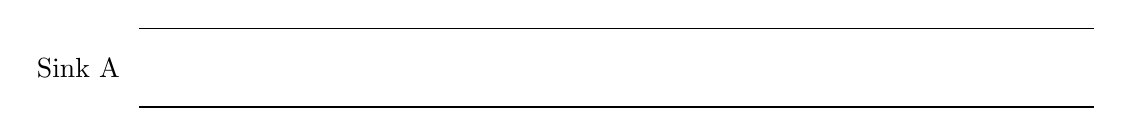
\begin{tikzpicture}


    \newcounter{numRails}
    \newcommand{\drawRail}[1]{
      \addtocounter{numRails}{1}
      
      \node [label=left:{#1}] (RailStart) at (0, 0.5) {};
      \draw (0, 1)  -- ++(\textwidth, 0);
      \draw (0, 0)  -- ++(\textwidth, 0);
    }
    \newcommand{\drawSyncPeriod}[3]{
        % #1 = start (x axis)
        % #2 = period length
        % #3 = number of periods
        \foreach \x in {1, ..., #3} {
            %\draw[arrows={-latex}] ({\x * #2}, 0) --++ ++(0, 1);
        }
    }
        
        
    \drawRail{Sink A}
    \drawSyncPeriod{0}{1}{3}

\end{tikzpicture}}


To get around this I added a timeout that restricts the amount of time the source can spend trying to analyse a specific
channel when there are other periods that need estimating.

The general case for determining a sink's period involves observing two of the sequence numbers ($n_1, n_2$) emitted by a sink,
recording the times they were observed ($r_1, r_2$) and then calculating:

$$t = \frac{r_2 - r_1} {n_1 - n_2}$$

This allows the period to be calculated without observing consecutive sequence numbers, however the two
sequence numbers must be observed within the same synchronisation phase. In the case where $n=1$ this is impossible,
so I added a special case that calculates

$$t = \frac{r_2 -r_1} {12}$$

When $n_2 > n_1$ we cannot reliably calculate the period as the second
sequence number may not be the sink's $n_max$, thus giving a larger $t$, which could cause us to transmit outside
of the reception period. In this instance $n1$ is replaced with $n_2$'s values and $n_2$ is reset.

\section{Clock Drift}

This is inevitable in systems without a centralised clock, especially when wireless communication is involved.
To help combat drift the source always performs calculations using times events were triggered at, rather than the
`current' time. After each broadcast the source schedules a new broadcast in $t * (11 + n)$ ticks and a resync in 
$(t * (10 + n)) - x$ ticks. The resync is used to verify that the estimated reception period is accurate.

\section{Power Saving}

My implementation saves power by scaling down the transmission power based on the signal strength of received packets.
Received power strength is between $0-255$ and transmission power $0-63$. Calculating min power needed to send to sink_X:

$$
\mathit{tx\_power}_x = \frac{\mathit{rx\_power}_x} {255} \times 63
$$

However using this exact value will mean a different min power is required as noise/distance from sink changes. To get around
this I transmit at double the minimum required power.

$$
\mathit{tx\_power}_x = max(63, \frac{\mathit{rx\_power}_x} {255} \times 63)
$$

The above operation can be approximated using multiplications of powers of 2, aka bit shifts.

\begin{align*}
\mathit{tx\_power}_x
&= \mathit{rx\_power}_x \times 2^{-8} \times 2^6 \\
&= \mathit{rx\_power}_x \times 2^{-2}
\end{align*}

Enabling power consumption tracing in the simulation allows us to monitor usage:

\missingfigure[]{Show the power consumption graph for before/after}


\end{document}

